\section{Derivation of a MOSFET Small Signal Model}
\begin{frame}{Derivation: Notational Conventions}
    \begin{itemize}
        \item DC quantities are labeled with UPPERCASE variables and UPPERCASE subindices: 
        $V_{\mathrm{GS}}$
        \item Pure AC quantities are labeled with lowercase variables and lowercase subindices: 
        $v_{\mathrm{gs}}$
        \item Superpositions of both quantities are labeled with lowercase variables and 
        UPPERCASE subindices: $v_{\mathrm{GS}}=V_{\mathrm{GS}}+v_{\mathrm{gs}}$

        \begin{figure}
            \centering
            \includegraphics[width=0.4\textwidth]{../plots/notational_convention.pdf}
            \caption{Notational conventions for DC and AC quantities.}
            \label{fig:signal_convention}
        \end{figure}
    \end{itemize}
\end{frame}

\begin{frame}{Derivation: MOSFET Current-Voltage Characteristics}
    \vspace{0.5cm}
    \begin{figure}
        \centering
        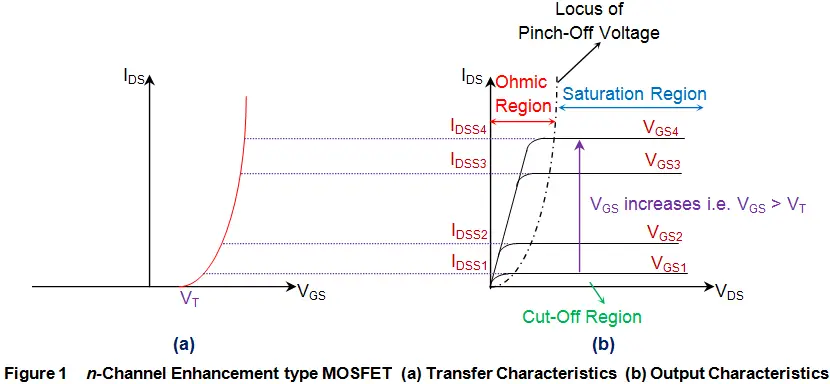
\includegraphics[width=0.7\textwidth]{../assets/mosfet_characteristics.png}
        \caption{MOSFET current-voltage characteristics.}
        \label{fig:mosfet_characteristics}
    \end{figure}
    \begin{itemize}
        \item Require saturation-region operation: $V_{\mathrm{DS}}\gg V_{\mathrm{GS}}-V_{\mathrm{t}}$
        \item In this regime, the following current-voltage characteristics are valid:
            \begin{itemize}
                \item $i_{\mathrm{drain}}=\frac{1}{2}k_{\mathrm{n}}(v_{\mathrm{gate}}-V_{\mathrm{t}})^{2}$
                \item $i_{\mathrm{gate}}=0$
            \end{itemize}
    \end{itemize}
\end{frame}

\begin{frame}{Derivation: Signal Current in Drain Terminal}
    \begin{itemize}
        \item Apply a signal $v_{\mathrm{GS}}=V_{\mathrm{GS}}+v_{\mathrm{gs}}$ to the gate terminal.
        \item This results in the following drain current:
    \end{itemize}
    \begin{align*}
        i_{\mathrm{D}}&=\frac{1}{2}k_{\mathrm{n}}(V_{\mathrm{GS}}+v_{\mathrm{gs}}
        -V_{\mathrm{t}})^{2} \\
        &=\underbrace{ \frac{1}{2}k_{\mathrm{n}}(V_{\mathrm{GS}}-V_{\mathrm{t}})^{2} }_{ =I_{\mathrm{D}}}+
        k_{\mathrm{n}}(V_{\mathrm{GS}}-V_{\mathrm{t}})v_{\mathrm{gs}}
        +\frac{1}{2}k_{\mathrm{n}}v_{\mathrm{gs}}^{2}
    \end{align*}
    \begin{itemize}
        \item The third term is negligible for sufficiently small $v_{\mathrm{gs}}$, i.e. 
        $v_{\mathrm{gs}}\ll 2(V_{\mathrm{GS}}-V_{\mathrm{t}})$.
        \item Neglecting the third term under the specified condition results in the following 
        expression for the drain current $i_{\mathrm{D}}$:
    \end{itemize}
    \begin{align*}
    i_{\mathrm{D}}&=I_{\mathrm{D}}+i_{\mathrm{d}} \\
    I_{\mathrm{D}}&=\frac{1}{2}k_{\mathrm{n}}(V_{\mathrm{GS}}-V_{\mathrm{t}})^{2} \\
    i_{\mathrm{d}}&=k_{\mathrm{n}}(V_{\mathrm{GS}}-V_{\mathrm{t}})v_{\mathrm{gs}}
    \end{align*}
    \begin{itemize}
        \item the parameter, that related $i_{\mathrm{d}}$ and $v_{\mathrm{gs}}$ is called the 
        transconductance $g_{\mathrm{m}}=k_{\mathrm{n}}(V_{\mathrm{GS}}-V_{\mathrm{t}})$ 
    \end{itemize}
\end{frame}